\documentclass{beamer}
\usetheme{default}
%\usetheme{pittsburgh}
\usecolortheme{albatross}

%###############################################################################
%#
%# Saját színek:
%#
\definecolor{todobgszin}{rgb}{0.64000,0.78000,0.22000}
\definecolor{todofrszin}{rgb}{0.00000,0.50000,0.00000}
\definecolor{background}{rgb}{0.00000,0.29412,0.49804}
%#
%###############################################################################

\setbeamercolor{normal text}{fg=white}
\setbeamertemplate{navigation symbols}{} % Navigációs ikonok off

\usepackage[T1]{fontenc}
\usepackage[utf8]{inputenc}
\usepackage[english,magyar]{babel}

\usepackage{hyperref}
\usepackage{color}
\usepackage{graphics}

\usebackgroundtemplate{

\includegraphics[width=\paperwidth, height=\paperheight]{figures/background.jpg}
}

% Néhány konstans deklarációja:
\newcommand{\vikszerzo}{\input{szerzok.inc}}
\newcommand{\vikkonzulens}{Ekler Péter Dr.}
\newcommand{\vikcim}{Hallgatói előrehaladás támogató ''badge'' rendszer}

%###############################################################################
%#
%# Footer definíció a szokásos címek beírásához.
%#
%# Csúnya hacket tartalmaz!!!
%# A "{footline}{#1}" utáni \textcolorral egy háttérszínnel megegyező "y"
%# karaktert írunk ki, hogy ne ugráljanak a dobozok a diákon.
%# Ha ez elmarad, akkor az alapvonal alá nyúló karaktereket (pl. g, y stb.)
%# tartalmazó stringek esetén eltérő magasságban lesz a footer, mint azoknál
%# amelyek csak az alapvonalra illeszkedő karaktereket tartalmaznak.
%#
\newcommand{\setfootline}[1]{\setbeamertemplate{footline}{\setbeamercolor{footline}{fg=white}\begin{beamercolorbox}[sep=1cm,wd=\textwidth,ht=1cm,left]{footline}{#1}\textcolor{background}{y}\end{beamercolorbox}}}
%#
%###############################################################################

%###############################################################################
%#
%# Saját eszközök:
%#
\newcommand{\todo}[1]{\fcolorbox{todofrszin}{todobgszin}{\emph{TODO: #1}}}
\newcommand{\angolul}[1]{\foreignlanguage{english}{#1}}
%#
%###############################################################################

\hypersetup{
    bookmarks=true,            % show bookmarks bar?
    unicode=true ,             % non-Latin characters in Acrobat’s bookmarks
    pdftitle={\vikcim},        % title
    pdfauthor={\vikszerzo},    % author
    pdfnewwindow=true,         % links in new window
    colorlinks=true,           % false: boxed links; true: colored links
    linkcolor=black,           % color of internal links
    citecolor=black,           % color of links to bibliography
    filecolor=black,           % color of file links
    urlcolor=black             % color of external links
}

\title{\vikcim}
\author{\vikszerzo \\ [0.5cm] \normalsize{Konzulens: \vikkonzulens}}
\date{2012. november 29.}

\begin{document}

\section{\vikcim}
\begin{frame}[plain]
\titlepage
\end{frame}

\section{A feladat leírása}
\setfootline{\todo{•} Gábor}
\begin{frame}[t]
\frametitle{A feladat leírása}
\small
A rendszer célja egy olyan webportál, ahol az oktatók felvihetnek úgynevezett feladatokat ami lehet egy adott tantárgy, önálló labor, kutató/fejlesztői munka stb. A feladatok felvitele mellett az oktatónak legyen lehetősége megfogalmazni célokat, amelynek elérésekor különféle ''badge''-t kaphat az adott hallgató. Például ha valaki elvégzett két mobilos tárgyat legalább 4-esre akkor automatikusan jár neki a ''mobile developer'' nevű badge. Minden ''badge'' mellé szöveges leírás és kép is feltölthető. Több badge kombinációja egy újabb, nagyobb badge-et is eredményezhet. A rendszer támogassa a hallgatók tárgy-elvégzésének könyvelését Neptun XML-ből is.

A rendszer különböztessen meg adminisztrátor és hallgató felhasználókat. Az adminisztrátorok lekérdezhessenek statisztikákat (legalább 3 grafikon). A hallgatók láthassák a megszerzett ''badge''-ket és az elérhető további ''badge''-ket, illetve azok feltételeit. A hallgatók nyomtathassanak (pl. PDF) egy saját profilt, melyen a megszerzett ''badge''-ik láthatók.

A weboldal feleljen meg a mai modern követelményeknek (AJAX, Form authentikáció stb.).
\end{frame}

\section{Architektúra - 3 réteg}
\setfootline{\todo{•} Gábor}
\begin{frame}[t]
\frametitle{Architektúra}
\begin{figure}[!ht]
\centering
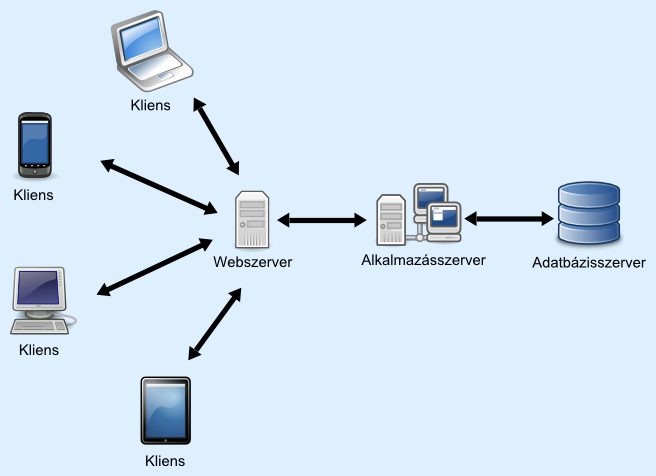
\includegraphics[width=90mm, keepaspectratio]{figures/3tier_simple_001.png}
\end{figure}
\end{frame}

\section{ER diagram}
\setfootline{\todo{•} Gábor}
\begin{frame}[t]
\frametitle{ER diagram}
\begin{figure}[!ht]
\centering
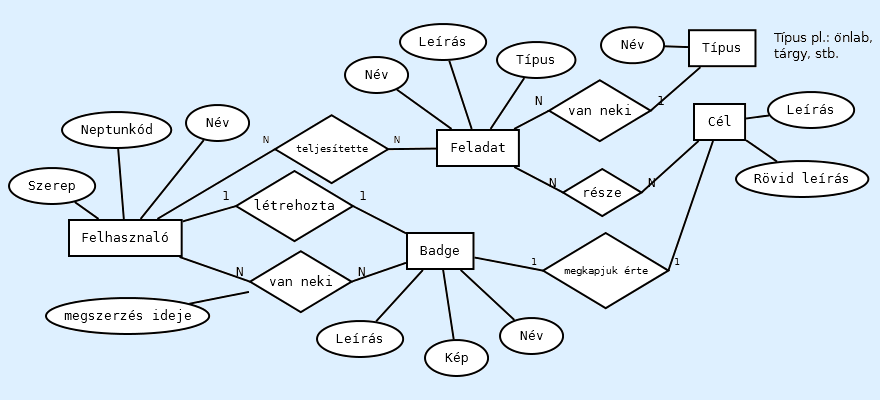
\includegraphics[width=110mm, keepaspectratio]{figures/modell.png}
\end{figure}
\end{frame}

\section{Use Case diagram}
\setfootline{\todo{•} Gábor}
\begin{frame}[t]
\frametitle{Use Case diagram}
\begin{figure}[!ht]
\centering
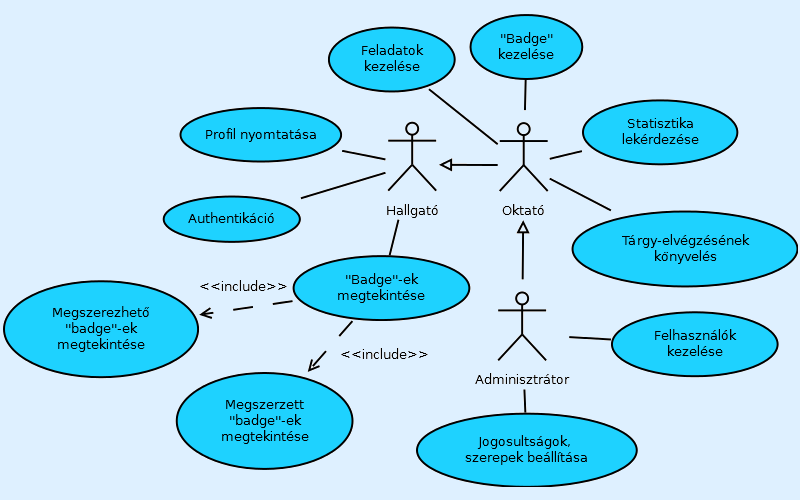
\includegraphics[width=110mm, keepaspectratio]{figures/use_case.png}
\end{figure}
\end{frame}

\section{Python}
\setfootline{\todo{•} Gyuri}
\begin{frame}[t]
\frametitle{Python}
\begin{itemize}
\item Egyszerű, könnyen olvasható
\item Bár szkript nyelv, mégis objektum orientált
\item Magasszintű, dinamikus adattípusok
\item Együttműködés más nyelvekkel (C, C++, Java, stb.)
\end{itemize}
\end{frame}

\section{Django}
\setfootline{\todo{•} Gyuri}
\begin{frame}[t]
\frametitle{Django}
\begin{itemize}
\item MVC architektúrájú Webes keretrendszer
\item Automatikus admin interfész
\item ORM
\end{itemize}
\end{frame}

\section{Admin felület}
\setfootline{\todo{•} Gyuri}
\begin{frame}[t]
\frametitle{Admin felület}
\begin{figure}[!ht]
\centering
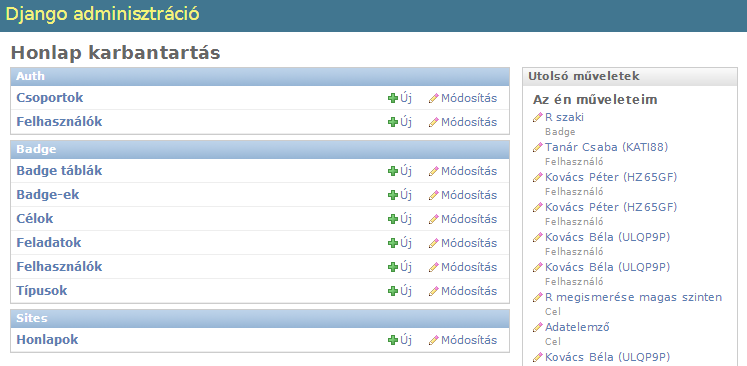
\includegraphics[width=110mm, keepaspectratio]{figures/admin.png}
\end{figure}
\end{frame}

\section{Oktatói oldal}
\setfootline{\todo{•} Gyuri}
\begin{frame}[t]
\frametitle{Oktatói oldal}
Elkészült funkciók:
\begin{itemize}
\item Típusok kezelése
\item Feladatok kezelése
\item Célok kezelése
\item Statisztika - Oktatók által létrehozott badge-ek száma
\end{itemize}
\begin{figure}[!ht]
\centering
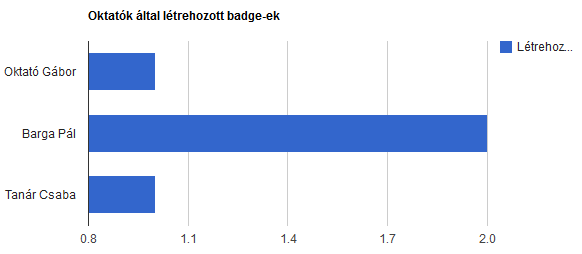
\includegraphics[width=90mm, keepaspectratio]{figures/stat.png}
\end{figure}
\end{frame}

\section{Hallgatói oldal}
\setfootline{\todo{•} Gyuri}
\begin{frame}[t]
\frametitle{Hallgatói oldal}
Elkészült funkciók:
\begin{itemize}
\item Összes badge listázása
\item Megszerzett badge-ek listázása
\end{itemize}
\end{frame}

\section{Hátralévő feladatok}
\setfootline{\todo{•} Gyuri}
\begin{frame}[t]
\frametitle{Hátralévő feladatok}
\end{frame}

\section{Kérdések}
\setfootline{\angolul{Is There Anybody Out There?}}
\begin{frame}[c]
\frametitle{}
\begin{center}
\huge{\textbf{Kérdések?}}\\
\begin{figure}[!ht]
\centering

\includegraphics[width=20mm, keepaspectratio]{figures/questions.png}
\end{figure}
\end{center}
\end{frame}

\section{Vége}
\setfootline{\angolul{Comfortably Numb}}
\begin{frame}[c]
\frametitle{}
\begin{center}
\huge{\textbf{Köszönjük a figyelmet!}}
\end{center}
\end{frame}

\end{document}
